% Main overview figure. Compile: pdflatex fig_overview.tex  (output is 3.3in wide)
\documentclass[border=0pt]{standalone}
\usepackage{mathptmx}
\usepackage{amsmath,amssymb}
\usepackage{tikz}
\usetikzlibrary{arrows.meta,calc}
\definecolor{acc}{RGB}{176,58,46}   % muted red  (dark in grayscale)
\definecolor{blu}{RGB}{52,101,164}  % muted blue
\begin{document}
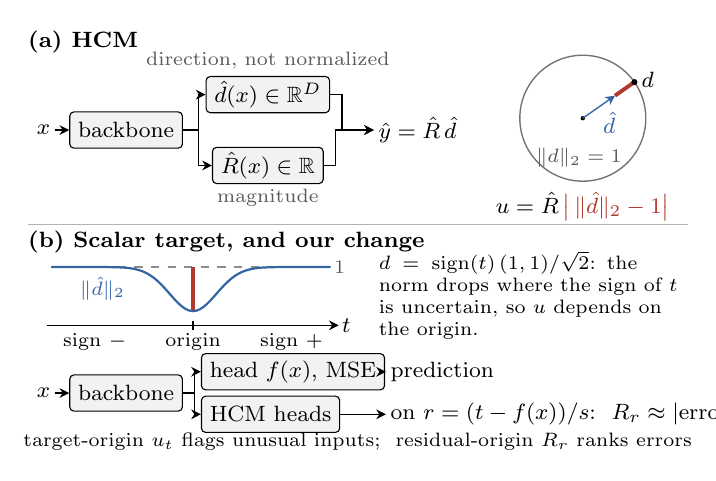
\begin{tikzpicture}[x=1cm,y=1cm,
  every node/.style={font=\fontsize{8}{9}\selectfont,inner sep=1.5pt},
  box/.style={draw,rounded corners=1.5pt,minimum height=0.46cm,inner xsep=3pt,fill=black!5},
  arr/.style={-{Stealth[length=3.5pt,width=3.5pt]},line width=0.5pt},
  sm/.style={font=\fontsize{7}{8}\selectfont}]
\path[use as bounding box] (0,0) rectangle (8.382,5.4);

% ---------------- (a) ----------------
\node[anchor=west,inner sep=0pt] at (0,5.22) {\textbf{(a) HCM}};
\node (x) at (0.2,4.1) {$x$};
\node[box] (bb) at (1.25,4.1) {backbone};
\node[box] (d) at (3.05,4.55) {$\hat d(x)\in\mathbb{R}^D$};
\node[box] (R) at (3.05,3.65) {$\hat R(x)\in\mathbb{R}$};
\node[sm,text=black!65] at (3.05,4.98) {direction, not normalized};
\node[sm,text=black!65] at (3.05,3.24) {magnitude};
\node (y) at (4.95,4.1) {$\hat y=\hat R\,\hat d$};
\draw[arr] (x) -- (bb);
\draw[arr] (bb.east) -- ++(0.2,0) |- (d.west);
\draw[arr] (bb.east) -- ++(0.2,0) |- (R.west);
\draw[arr] (d.east) -- ++(0.15,0) |- (y.west);
\draw[arr] (R.east) -- ++(0.15,0) |- (y.west);
% unit circle
\coordinate (c) at (7.05,4.25);
\draw[black!55,line width=0.5pt] (c) circle (0.8);
\fill (c) circle (0.8pt);
\draw[line width=1.4pt,acc] ($(c)+(35:0.5)$) -- ($(c)+(35:0.8)$);
\draw[arr,blu] (c) -- ($(c)+(35:0.5)$);
\fill ($(c)+(35:0.8)$) circle (1.1pt);
\node[anchor=west] at ($(c)+(35:0.84)$) {$d$};
\node[anchor=north,blu] at ($(c)+(22:0.36)$) {$\hat d$};
\node[sm,text=black!65] at ($(c)+(-0.05,-0.5)$) {$\|d\|_2=1$};
\node at (7.05,3.13) {$u=\hat R\,{\color{acc}\bigl|\,\|\hat d\|_2-1\bigr|}$};

\draw[black!30,line width=0.4pt] (0,2.9) -- (8.382,2.9);

% ---------------- (b) ----------------
\node[anchor=west,inner sep=0pt] at (0,2.68) {\textbf{(b) Scalar target, and our change}};
% number line with the norm curve
\draw[arr] (0.25,1.62) -- (3.95,1.62) node[anchor=west,inner sep=1pt] {$t$};
\draw (2.1,1.56) -- (2.1,1.68);
\node[sm,anchor=north] at (2.1,1.58) {origin};
\node[sm,anchor=north] at (0.85,1.58) {sign $-$};
\node[sm,anchor=north] at (3.35,1.58) {sign $+$};
\draw[black!45,dashed,line width=0.4pt] (0.3,2.36) -- (3.85,2.36);
\node[sm,anchor=west,text=black!65,inner sep=1pt] at (3.85,2.36) {1};
\draw[blu,line width=0.8pt,domain=0.3:3.85,samples=80]
  plot (\x,{2.36-0.56*exp(-((\x-2.1)/0.42)^2)});
\draw[acc,line width=1.4pt] (2.1,1.82) -- (2.1,2.36);
\node[sm,blu,anchor=north,inner sep=1pt] at (0.95,2.28) {$\|\hat d\|_2$};
\node[sm,anchor=west,text width=3.8cm,align=left] at (4.4,2.0)
  {$d=\mathrm{sign}(t)\,(1,1)/\sqrt2$: the norm drops where the sign of $t$ is uncertain, so $u$ depends on the origin.};
% our variant
\node (x2) at (0.2,0.76) {$x$};
\node[box] (bb2) at (1.25,0.76) {backbone};
\node[box,anchor=west] (f) at (2.2,1.03) {head $f(x)$, MSE};
\node[box,anchor=west] (h) at (2.2,0.49) {HCM heads};
\node[anchor=west] (pr) at (4.55,1.03) {prediction};
\node[anchor=west] (rr) at (4.55,0.49) {on $r=(t-f(x))/s$:\ \ $R_r\approx|\text{error}|$};
\draw[arr] (x2) -- (bb2);
\draw[arr] (bb2.east) -- ++(0.15,0) |- (f.west);
\draw[arr] (bb2.east) -- ++(0.15,0) |- (h.west);
\draw[arr] (f.east) -- (pr.west);
\draw[arr] (h.east) -- (rr.west);
\node[sm,anchor=south,inner sep=0pt] at (4.19,0.02) {target-origin $u_t$ flags unusual inputs;\ \ residual-origin $R_r$ ranks errors};
\end{tikzpicture}
\end{document}
